\documentclass[,12pt]{article}
\usepackage{geometry}
\geometry{margin=1in,top=.5in,bottom=1in}
\usepackage{epsfig}
\usepackage{graphicx}
\usepackage{rotating}
\usepackage{url}
\usepackage{chicago}
\bibliographystyle{chicago}
\newcommand{\Robject}[1]{{\texttt{#1}}}
\newcommand{\Rfunction}[1]{{\texttt{#1}}}
\newcommand{\Rpackage}[1]{{\textit{#1}}}
\newcommand{\Rclass}[1]{{\textit{#1}}}
\newcommand{\Rmethod}[1]{{\textit{#1}}}
\newcommand{\Rfunarg}[1]{{\textit{#1}}}
%\VignetteIndexEntry{clustvarsel Overview}
%\VignetteDepends{mclust02}
%\VignetteKeywords{Variable selection, Feature selection, Model-based clustering}
%\VignettePackage{clustvarsel}

\usepackage{/Library/Frameworks/R.framework/Resources/share/texmf/Sweave}
\begin{document}
\title{The Variable Selection for Model-based Clustering (\Rpackage{clustvarsel}) package}
\author{Nema Dean}
\date{17th March 2006}
\maketitle
\tableofcontents

\section{Overview} 

The \Rpackage{clustvarsel} package can be used to find the (locally) optimal subset of variables with group/cluster information in a dataset with continuous variables. 

Each variable's evidence for being useful for clustering given the currently selected clustering variables is given by the difference between the BIC for the model with clustering (allowed to vary over 2 to a maximum number of groups and any of the different covariance parameterizations allowed in mclust02) using the set of clustering variables including the variable being checked and the sum of BICs for the model with clustering (allowed to vary over 2 to a maximum number of groups and any of the different covariance parameterizations allowed in mclust02) using the set of clustering variables without the variable being checked and the model for the variable being checked being conditionally independent of the clustering given the other clustering variables (this is modeled as a regression of the variable being checked on the other clustering variables).  

For more details on the model see \citeN{raftery04}, for an overview of model-based clustering see \citeN{FraleyRaftery2002} and for more details on the \Rpackage{mclust02} package see \citeN{fraley02} or \url{http://www.stat.washington.edu/mclust/}.

Two different search algorithms are available for checking single variables for inclusion into/exclusion from the set of selected clustering variables. The \Rfunarg{``greedy''} search option checks at every inclusion step the inclusion of each single variable not currently selected into the current set of selected clustering variables. The variable that has highest evidence of inclusion is proposed and, if its clustering evidence is stronger than the evidence against clustering it is included. At every exclusion step  the \Rfunarg{``greedy''} search option checks the exclusion of each single variable in the currently selected set of clustering variables and proposes the variable that has lowest evidence of clustering. The proposed variable is removed if its evidence of clustering is weaker than its evidence against clustering.This is similar to the idea for stepwise regression and may suffer from the same instabilities mentioned in \citeN{miller90} inherent in that approach (although this has not been apparent in the simulations and examples tried thus far).

The \Rfunarg{``headlong''} search (see \citeN{badsberg92} for full details) involves potentially checking less variables at each inclusion or exclusion step and so may be quicker than the \Rfunarg{``greedy''} search (if possibly less optimal) for use on datasets with a large number of variables. 

At each inclusion step, the algorithm only checks single variables not currently in the set of clustering variables up until the difference between the BIC for clustering versus not clustering is above a prespecified level \Rfunarg{upper} (the default is 0, i.e. where evidence for clustering is greater than that for not clustering by any amount). Because the algorithm will stop once this criterion is satisfied it will not necessarily check all the variables available and the variable selected will not necessarily be the best possible variable at that step. Any variables who are checked during this step, whose difference between the BIC for clustering versus not clustering is below a prespecified level \Rfunarg{lower} (the default is -10, i.e. whose evidence is strongly against clustering) are removed from consideration for the rest of the algorithm. Because of this, possibly irrelevant variables can be removed early on in the algorithm and further reduce the number of variables checked at each step. Similarly at each exclusion, the algorithm only checks single variables currently in the set of clustering variables up until the difference the BIC for clustering versus not clustering is below the same prespecified level \Rfunarg{upper}. The algorithm stops checking once a variable satisfies this criterion and that variable is removed from the set. If the difference in BIC is smaller than \Rfunarg{lower} the variable is removed from consideration for the rest of the algorithm, otherwise it can still be checked in future inclusion/exclusion steps. 

The speed/optimally tradeoff can be changed by increasing or decreasing the different levels, e.g. by setting \Rfunarg{upper} to 10 instead of 0 we require a variable to have stronger evidence of clustering before it is included and by setting \Rfunarg{lower} to 0 we remove variables that at any stage have evidence of clustering weaker by any amount than evidence against clustering.

\section{Main \Rfunction{clustvarsel} function}
We begin by loading the package (the required \Rpackage{mclust02} package will automatically be loaded at the same time).
\begin{Schunk}
\begin{Sinput}
> library(clustvarsel)
\end{Sinput}
\end{Schunk}

The basic \Rfunction{clustvarsel}  function has the default settings of using the \Rfunarg{``greedy''} search, not using a subset for the hierarchical clustering phase of cluster model fitting, allowing an equal covariances hierarchical model when variable covariances model gives no viable answers, automatically selecting the first two variables regardless of whether the evidence of univariate/bivariate clustering is greater than not clustering (to provide starting variables) and a maximum number of paired inclusion and exclusion steps of 100. The default options for allowing different covariance parameterizations for both univariate clustering in \Rfunarg{emModels1} and multivariate clustering in \Rfunarg{emModels2} are all possible parameterizations currently available in \Rpackage{mclust02} (see the help file for \Rfunction{EMclust} for more details).

The only inputs required are a matrix \Rfunarg{X} of continuous data with rows corresponding to observations and columns (at least 2) corresponding to variables and the maximum number of groups \Rfunarg{G} believed to be possible in the data.

For our example we will use the crabs data in the \Rpackage{MASS} package. We know that there are 50 observations for each class (blue males, blue females, orange males and orange females) that are in order so we create a vector \Robject{crabscl}, identifying the true classification of the observations. We create our data matrix X and look at the pairs plot of the data.

\begin{Schunk}
\begin{Sinput}
> library(MASS)
> data(crabs)
> X <- crabs[, 4:8]
> colnames(X)
\end{Sinput}
\begin{Soutput}
[1] "FL" "RW" "CL" "CW" "BD"
\end{Soutput}
\begin{Sinput}
> pairs(X)
> crabscl <- c(rep(1, 50), rep(2, 50), rep(3, 50), rep(4, 50))
\end{Sinput}
\end{Schunk}
The pairs plot for X is given in Figure \ref{plot1}.
First we look at the result from choosing the best model in terms of BIC for clustering on all variables allowing all possible parameterizations and the number of groups to range over 1 to 5 (our maximum number of possible clusters \Rfunarg{G} in the dataset). We cluster the data using \Rfunction{EMclust} from the \Rpackage{mclust02} and look at the results using the \Rfunction{summary} function. We then extract the estimated classifications from the best model in terms of BIC from the summary and use \Rfunction{classError} to look at the misclassification error between the current and true classifications. We can use \Rfunction{table} to look at the cross tabulated classifications.
 
\begin{Schunk}
\begin{Sinput}
> clust1 <- EMclust(X, G = 1:5)
> summary(clust1, X)
\end{Sinput}
\begin{Soutput}
classification table:

 1  2  3 
75 77 48 

uncertainty (quartiles):
          0%          25%          50%          75%         100% 
0.000000e+00 1.171732e-07 1.853438e-03 2.770624e-02 4.892871e-01 

best BIC values:
    EEV,3     EEV,4     EEE,3 
-2925.590 -3016.711 -2933.521 

best model: ellipsoidal, equal volume and shape 
\end{Soutput}
\begin{Sinput}
> cl1 <- summary(clust1, X)$class
> classError(cl1, crabscl)
\end{Sinput}
\begin{Soutput}
[1] 0.375
\end{Soutput}
\begin{Sinput}
> table(cl1, crabscl)
\end{Sinput}
\begin{Soutput}
   crabscl
cl1  1  2  3  4
  1 25 50  0  0
  2  0  0 27 50
  3 25  0 23  0
\end{Soutput}
\end{Schunk}
Now we run the algorithm to automatically select which variables in the dataset are truly useful for clustering using \Rfunction{clustvarsel} and look at the steps of the algorithm. We then create \Robject{S}, the matrix of the selected variables and check which variables are in it.

\begin{Schunk}
\begin{Sinput}
> result <- clustvarsel(X, G = 5)
> result$steps.info
\end{Sinput}
\begin{Soutput}
     Variable proposed BIC of new clustering variables set BIC difference     
[1,] "CW"              "-1408.72243051261"                 "-6.23030510251988"
[2,] "RW"              "-1908.96423491868"                 "127.398162308462" 
[3,] "FL"              "-2357.17088014855"                 "81.3271493966722" 
[4,] "FL"              "-2357.17088014855"                 "81.3271493966722" 
[5,] "BD"              "-2609.88963370441"                 "55.8879054648505" 
[6,] "BD"              "-2609.88963370441"                 "55.8879054648505" 
[7,] "CL"              "-2609.88963370441"                 "-107.399613408393"
[8,] "BD"              "-2609.88963370441"                 "55.8879054648505" 
     Type of step Decision  
[1,] "Add"        "Accepted"
[2,] "Add"        "Accepted"
[3,] "Add"        "Accepted"
[4,] "Remove"     "Rejected"
[5,] "Add"        "Accepted"
[6,] "Remove"     "Rejected"
[7,] "Add"        "Rejected"
[8,] "Remove"     "Rejected"
\end{Soutput}
\begin{Sinput}
> S <- result$sel.var
> colnames(S)
\end{Sinput}
\begin{Soutput}
[1] "CW" "RW" "FL" "BD"
\end{Soutput}
\end{Schunk}
Next we look at the results from clustering (using \Rfunction{EMclust}) on S using the \Rfunction{summary} command. Again we extract the classifications from this model, \Robject{cl2} and use \Rfunction{classError} and \Rfunction{table} to look at the misclassifications comparing it to the true classifications  and the classifications from the model with all variables, \Robject{cl1}.

\begin{Schunk}
\begin{Sinput}
> clust2 <- EMclust(S, G = 1:5)
> summary(clust2, S)
\end{Sinput}
\begin{Soutput}
classification table:

 1  2  3  4 
60 40 45 55 

uncertainty (quartiles):
          0%          25%          50%          75%         100% 
0.000000e+00 1.878522e-08 4.637432e-05 1.225672e-02 4.964781e-01 

best BIC values:
    EEV,4     EEV,5     VVV,4 
-2609.890 -2760.546 -2731.526 

best model: ellipsoidal, equal volume and shape 
\end{Soutput}
\begin{Sinput}
> cl2 <- summary(clust2, S)$class
> classError(cl2, crabscl)
\end{Sinput}
\begin{Soutput}
[1] 0.075
\end{Soutput}
\begin{Sinput}
> table(cl2, crabscl)
\end{Sinput}
\begin{Soutput}
   crabscl
cl2  1  2  3  4
  1 10 50  0  0
  2 40  0  0  0
  3  0  0  0 45
  4  0  0 50  5
\end{Soutput}
\begin{Sinput}
> table(cl1, cl2)
\end{Sinput}
\begin{Soutput}
   cl2
cl1  1  2  3  4
  1 60 15  0  0
  2  0  0 45 32
  3  0 25  0 23
\end{Soutput}
\end{Schunk}
\section{Adjustments for Speeding Up Algorithm}
If we have a large number of observations in our dataset we allow \Rfunction{EMclust} to use only a subset of the data at the computationally expensive hierarchical stage of clustering to speed up the algorithm. We construct a medium sized dataset below for which we compare the time between using a subset (setting \Rfunarg{samp} to TRUE) of 200 observations (setting \Rfunarg{sampsize} to 200) and using all observations for the hierarchical clustering stage.

We set up the 4 dimensional data matrix X with clustering information only in the first two variables and define the mixing proportion \Robject{pro}, the two cluster means \Robject{mu1} and \Robject{mu2} and the two cluster covariances \Robject{sigma1} and \Robject{sigma2}. We then simulate from the model with these parameters and simulate independent normally distributed noise for the remaining two variables. We then use the function \Rfunction{system.time} to measure the time taken to run \Rfunction{clustvarsel} with a sample of 200 (\Rfunarg{samp}=T, \Rfunarg{sampsize}=200) and without sampling. Finally we check to make sure both selected the correct variables.

\begin{Schunk}
\begin{Sinput}
> X <- matrix(0, 400, 4)
> pro <- 0.5
> mu1 <- c(0, 0)
> mu2 <- c(3, 3)
> sigma1 <- matrix(c(1, 0.5, 0.5, 1), 2, 2, byrow = TRUE)
> sigma2 <- matrix(c(1.5, -0.7, -0.7, 1.5), 2, 2, byrow = TRUE)
> u <- runif(400)
> library(MASS)
> for (i in 1:400) {
+     ifelse(u[i] < pro, X[i, 1:2] <- mvrnorm(1, mu1, sigma1), 
+         X[i, 1:2] <- mvrnorm(1, mu2, sigma2))
+ }
> X[, 3] <- rnorm(400, 1.5, 2)
> X[, 4] <- rnorm(400, 2, 1)
> system.time(result1 <- clustvarsel(X, G = 3, samp = T, sampsize = 200))
\end{Sinput}
\begin{Soutput}
[1]  6.154  0.177 16.074  0.000  0.000
\end{Soutput}
\begin{Sinput}
> system.time(result2 <- clustvarsel(X, G = 3))
\end{Sinput}
\begin{Soutput}
[1]  7.144  0.212 22.668  0.000  0.000
\end{Soutput}
\begin{Sinput}
> colnames(result1$sel.var)
\end{Sinput}
\begin{Soutput}
[1] "2" "1"
\end{Soutput}
\begin{Sinput}
> colnames(result2$sel.var)
\end{Sinput}
\begin{Soutput}
[1] "2" "1"
\end{Soutput}
\end{Schunk}
If we have a large number of variables in our dataset we may find that using the \Rfunarg{``headlong''}  search algorithm option may be faster than the default \Rfunarg{``greedy''} search. We construct a medium sized dataset below for which we compare the time between using the headlong method (search=\Rfunarg{``headlong''}) and using the greedy method.


We set up the 8 dimensional data matrix X with clustering information only in the last two variables and define the mixing proportion \Robject{pro}, the two cluster means \Robject{mu1} and \Robject{mu2} and the two cluster covariances \Robject{sigma1} and \Robject{sigma2}. We then simulate from the model with these parameters and simulate independent and multivariate normally distributed noise for the remaining six variables. We then use the function \Rfunction{system.time} to measure the time taken to run \Rfunction{clustvarsel} with headlong search (\Rfunarg{search}=``headlong'') versus greedy search (the default). Finally we check to make sure both selected the correct variables. We can also speed up the algorithm by restricting the models checked to equal and unconstrained covariances (\Rfunarg{emModels2}=c("EEE","VVV")).

\begin{Schunk}
\begin{Sinput}
> X <- matrix(0, 200, 8)
> pro <- 0.5
> mu1 <- c(0, 0)
> mu2 <- c(3, 3)
> sigma1 <- matrix(c(1, 0.5, 0.5, 1), 2, 2, byrow = TRUE)
> sigma2 <- matrix(c(1.5, -0.7, -0.7, 1.5), 2, 2, byrow = TRUE)
> u <- runif(200)
> library(MASS)
> for (i in 1:200) {
+     ifelse(u[i] < pro, X[i, 7:8] <- mvrnorm(1, mu1, sigma1), 
+         X[i, 7:8] <- mvrnorm(1, mu2, sigma2))
+ }
> X[, 1] <- rnorm(200, 1.5, 2)
> X[, 2] <- rnorm(200, 2, 1)
> X[, 3:4] <- mvrnorm(200, mu1, sigma1)
> X[, 5:6] <- mvrnorm(200, mu2, sigma2)
> system.time(result1 <- clustvarsel(X, G = 3, search = "headlong"))
\end{Sinput}
\begin{Soutput}
[1]  3.999  0.121 11.818  0.000  0.000
\end{Soutput}
\begin{Sinput}
> system.time(result2 <- clustvarsel(X, G = 3))
\end{Sinput}
\begin{Soutput}
[1]  7.439  0.185 17.731  0.000  0.000
\end{Soutput}
\begin{Sinput}
> colnames(result1$sel.var)
\end{Sinput}
\begin{Soutput}
[1] "7" "8"
\end{Soutput}
\begin{Sinput}
> colnames(result2$sel.var)
\end{Sinput}
\begin{Soutput}
[1] "7" "8"
\end{Soutput}
\begin{Sinput}
> system.time(result3 <- clustvarsel(X, G = 3, emModels2 = c("EEE", 
+     "VVV"), search = "headlong"))
\end{Sinput}
\begin{Soutput}
[1] 2.540 0.078 7.031 0.000 0.000
\end{Soutput}
\begin{Sinput}
> colnames(result3$sel.var)
\end{Sinput}
\begin{Soutput}
[1] "7" "8"
\end{Soutput}
\end{Schunk}
If we have both a large number of observations and variables we can use both the \Rfunarg{samp} and \Rfunarg{``headlong''} options. Again we generate an 8 dimensional data matrix X in a similar way to the previous example, this time with 400 observations. We then use \Rfunction{system.time} to compare the time taken for variable selection with the models checked restricted to equal and unconstrained covariances (\Rfunarg{emModels2}=c("EEE","VVV")), ``\Rfunarg{headlong}'' search and sampling 200 observations for the hierarchical clustering stage (\Rfunarg{samp}=T and \Rfunarg{sampsize}=200) versus variable selection just with \Rfunarg{headlong} search and variable selection with \Rfunarg{greedy} search. 

\begin{Schunk}
\begin{Sinput}
> X <- matrix(0, 400, 8)
> pro <- 0.5
> mu1 <- c(0, 0)
> mu2 <- c(3, 3)
> sigma1 <- matrix(c(1, 0.5, 0.5, 1), 2, 2, byrow = TRUE)
> sigma2 <- matrix(c(1.5, -0.7, -0.7, 1.5), 2, 2, byrow = TRUE)
> u <- runif(400)
> library(MASS)
> for (i in 1:400) {
+     ifelse(u[i] < pro, X[i, 7:8] <- mvrnorm(1, mu1, sigma1), 
+         X[i, 7:8] <- mvrnorm(1, mu2, sigma2))
+ }
> X[, 1] <- rnorm(400, 1.5, 2)
> X[, 2] <- rnorm(400, 2, 1)
> X[, 3:4] <- mvrnorm(400, mu1, sigma1)
> X[, 5:6] <- mvrnorm(400, mu2, sigma2)
> system.time(result1 <- clustvarsel(X, G = 3, emModels2 = c("EEE", 
+     "VVV"), search = "headlong", samp = T, sampsize = 200))
\end{Sinput}
\begin{Soutput}
[1]  5.420  0.190 16.108  0.000  0.000
\end{Soutput}
\begin{Sinput}
> system.time(result2 <- clustvarsel(X, G = 3, search = "headlong"))
\end{Sinput}
\begin{Soutput}
[1] 10.567  0.330 25.471  0.000  0.000
\end{Soutput}
\begin{Sinput}
> system.time(result3 <- clustvarsel(X, G = 3))
\end{Sinput}
\begin{Soutput}
[1] 17.827  0.480 48.359  0.000  0.000
\end{Soutput}
\begin{Sinput}
> colnames(result1$sel.var)
\end{Sinput}
\begin{Soutput}
[1] "8" "7"
\end{Soutput}
\begin{Sinput}
> colnames(result2$sel.var)
\end{Sinput}
\begin{Soutput}
[1] "8" "7"
\end{Soutput}
\begin{Sinput}
> colnames(result3$sel.var)
\end{Sinput}
\begin{Soutput}
[1] "8" "7"
\end{Soutput}
\end{Schunk}
\bibliography{refs}

\begin{figure}[htbp]
\begin{center}
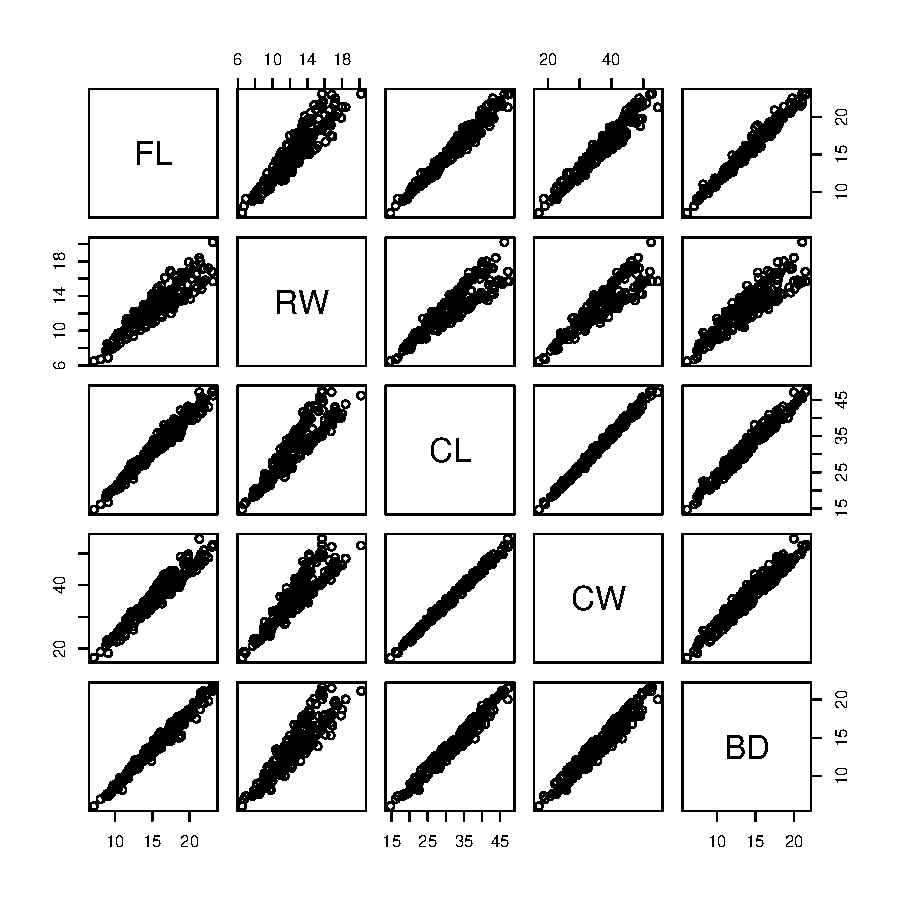
\includegraphics[height=6in,width=4in]{vignplot1}
\end{center}
\caption{Pairs plot of the crabs data}
\label{plot1}
\end{figure}
\end{document}
